\addcontentsline{toc}{chapter}{Network Layer}
\chapter*{\begin{center}Network Layer\end{center}}
\begin{center}(Layer 3 nello stack TCP/IP)\end{center}
\hrulefill \\

\noindent Per iniziare, il Network Layer può essere diviso in due macro-componenti che interagiscono fra di loro: \index{plane!data}\index{plane!control}Data Plane e Control Plane (dove Plane significa piano, strato). A questo layer dello stack, la PDU si chiama Datagramma.\index{datagramma}\\

\noindent Nel Data Plane vengono trattate tutte le funzioni \openapex pre-router'', incluso il tradizionale IP Forwarding che vedremo a breve.\\

\noindent Forwarding VS Routing:\index{forwarding}\index{routing}
\begin{itemize}
    \item Forwarding: azione svolta dal router, consiste nel trasferire un pacchetto da una input link interface alla opportuna output link interface;
    \item Routing: azione svolta a livello di rete, comprende TUTTO il processo per determinare il percorso (path) che il pacchetto percorre da mittente al destinatario.
\end{itemize}
\noindent N.B.: i protocolli di routing $\neq$ protocolli routabili\index{protocollo!routabile} ($\approx$ instradabili\footnote{protocollo utilizzato per mandare dati attraverso più reti, selezionando i formati dati opportuni in base alle reti in questione. Tipo IP. IP non decide nulla a livello di percorsi attraverso la rete (non è un protocollo di routing, ma routabile).}). Also, in internet non esistono (e non possono esistere) due indirizzi uguali corrispondenti a due diversi Host.\\

\addcontentsline{toc}{section}{IP}
\section*{\textcolor{WildStrawberry}{IP}}
\index{IP}
\underline{I}nternet \underline{P}rotocol\\

\noindent Definisce il modo in cui i pacchetti sono instradati.\\
\addcontentsline{toc}{subsection}{Datagramma IPv4}
\subsection*{Datagramma IPv4}
\index{IPv4}
\index{IPv4!datagramma}

\begin{figure} [h]
    \centering
    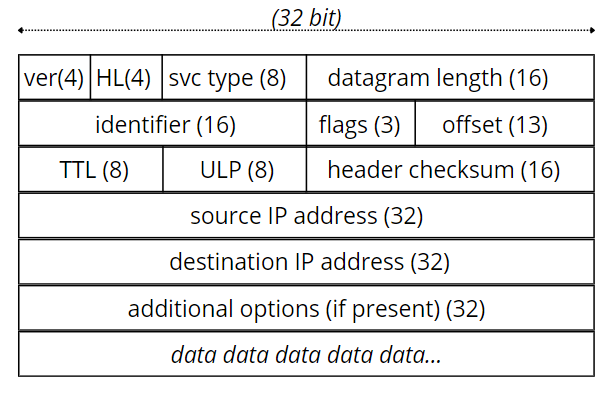
\includegraphics[width=0.5\linewidth]{Figures/04/headerIPv4.png}
    \caption{Struttura di un header IPv4. Tra parentesi sono indicati i bit di lunghezza di ciascun campo.}
    \label{fig:headipv4}

\end{figure}

\noindent In Figura \ref{fig:headipv4} è raffigurata la struttura di un header (intestazione) a livello di rete, nello specifico un header IP, versione 4 (esiste anche IPv6, lo vedremo brevemente più avanti). Le varie sigle stanno per:
\begin{itemize}
    \item ver: \textit{versione;}
    \item HL: \textit{header length}, lunghezza header;
    \item svc type: \textit{service type;}
    \item TTL: \textit{Time-To-Live;}
    \item ULP: \textit{Upper Layer Protocol,} ovvero che protocollo aspettarsi al layer immediatamente superiore (i.e., il layer di trasporto, quindi solitamente TCP o UDP);
\end{itemize}

\noindent N.B.: il time-to-live, sebbene esprima un concetto di \openapex tempo'', non è un valore da intendersi come un timer di ore e minuti, una cosa tipo \textit{hh:mm:ss}: è una unità di tempo \textit{logica}, ovvero un contatore a $n$ che viene decrementato di 1 ogni volta che un pacchetto arriva ad un router\footnote{Per capirci, invece di contare quanto tempo impiegate per arrivare dalla porta del bagno a quella della cucina, contate i passi che fate. I passi, coi piedi, i passi fisici.}. Se il TTL arriva a $=0$, allora il pacchetto viene dichiarato morto: questo per evitare che i pacchetti entrino per errore in circolo all'infinito tra i vari router della rete.\\

\noindent IPv6,\index{IPv6} come datagramma, è molto simile a IPv4 ma con qualche differenza, la più rilevante credo sia nelle dimensioni dell'indirizzo - non più 32 ma 128 bit - ed altre differenze nei contenuti.\footnote{Da qualche parte che non so dirvi al momento, esistono tools e metodi per convertire un indirizzo IPv4 in IPv6 e viceversa. Penso basti andarseli a cercare sul web.}\\

\noindent Interfaccia di rete\index{rete!interfaccia}: punto di connessione tra host e router (e.g.: una scheda Bluetooth, Ethernet, etc.). Ciascuna interfaccia di rete può avere più IP Address associati.\\

\addcontentsline{toc}{subsection}{Indirizzamenti}
\subsection*{Evoluzione degli Indirizzamenti}
\noindent Ovvero, piccolo excursus storico.\\

\begin{itemize}
    \item 1981 - Indirizzamento a 2 livelli \underline{classful}\index{indirizzi!classful}: semplice da comprendere e implementare, questo tipo di addressing architecture si basa sulla divisione in 5 classi di indirizzi, basate sui primi 4 bit dell'indirizzo IPv4. In questa architettura 2-layer classful, la struttura dell'indirizzo IP era: \begin{verbatim}
        (network_ID).(host_ID)
    \end{verbatim}
    la prima metà dell'indirizzo identificava la rete, la seconda metà l'host. Quindi la classe (identificata nei primi 4 bit a sinistra) è associata alla rete!

\begin{table}[h]
\centering
\begin{tabular}{cc}
classe                                                                                                         & \multicolumn{1}{l}{start address (decimale e binario)}                                            \\ \hline
\multicolumn{1}{|c|}{classe A}                                                                                 & \multicolumn{1}{c|}{\begin{tabular}[c]{@{}c@{}}0.0.0.0\\ \hl{0000}0000.00000000. (...)\end{tabular}}   \\ \hline
\multicolumn{1}{|c|}{classe B}                                                                                 & \multicolumn{1}{c|}{\begin{tabular}[c]{@{}c@{}}128.0.0.0\\ \hl{1000}000.00000000. (...)\end{tabular}}  \\ \hline
\multicolumn{1}{|c|}{classe C}                                                                                 & \multicolumn{1}{c|}{\begin{tabular}[c]{@{}c@{}}192.0.0.0\\ \hl{1100}0000.00000000. (...)\end{tabular}} \\ \hline
\multicolumn{1}{|c|}{\begin{tabular}[c]{@{}c@{}}classe D\\ \textit{(multicast)}\end{tabular}} & \multicolumn{1}{c|}{\begin{tabular}[c]{@{}c@{}}224.0.0.0\\ \hl{1110}0000.00000000. (...)\end{tabular}} \\ \hline
\multicolumn{1}{|c|}{\begin{tabular}[c]{@{}c@{}}classe E\\ \textit{(reserved)}\end{tabular}}  & \multicolumn{1}{c|}{\begin{tabular}[c]{@{}c@{}}240.0.0.0\\ \hl{1111}0000.00000000. (...)\end{tabular}} \\ \hline
\end{tabular}
\end{table}

    Questo sistema 2-layer classful è deprecato, non più in uso, ma talvolta viene chiesto all'esame, quindi il mio consiglio spassionato è: esercitatevi a convertire i numeri dal decimale al binario o memorizzate i numeri che delimitano le classi (0, 128, 192, 224 e 240. Gli intervalli, naturalmente, sono $0\div127$, $128\div191$, $192\div223$, $224\div239$ e $240\div255$.);
\item 1984 - Indirizzamento a 3 livelli classful: la struttura dell'indirizzo non è più: \begin{verbatim}
        (network_ID).(host_ID)
    \end{verbatim}
ma cambia in: \begin{verbatim}
        (network_ID).(subnet_ID).(host_ID)
    \end{verbatim}

Il subnetting è un argomento che vedremo tra un attimo;
\item 1993 - CIDR (Classless Inter-Domaining Routing)\index{CIDR}: viene eliminata la divisione in classi; indirizzi vengono gestiti in modo efficiente per fare routing a questa maniera \begin{verbatim}
    IP = < prefisso, suffisso >
\end{verbatim} 
dove il prefisso indica la rete e il suffisso indica l'host connesso alla rete. È una forma di subnetting\index{subnetting}, la dimensione di questi due campi varia arbitrariamente! Per risalire a dove inizia uno e dove finisce l'altro, per distinguerli tra di loro occorre usare un'altra stringa di bit chiamata \hl{maschera di rete} (netmask): la netmask\index{netmask}\index{rete!maschera} è una stringa di 32 bit disposti in una sequenza di $x$ bit \openapex 1'' seguiti da $y$ volte \openapex 0'' (ovviamente, $x+y$ deve tornare 32), tipo:
\begin{verbatim}
    11111111.11111111.11111111.00000000
\end{verbatim}
\noindent questo è il caso di una netmask $/24$ (cosiddetta \textit{barra 24,} ovvero, 24 bit `1' seguiti da 8 bit `0').
Facendo l'operazione di AND logico tra la netmask e l'indirizzo CIDR, possiamo separare la parte di rete dalla parte di host (rispettivamente nel prefisso e suffisso).
\end{itemize}

\noindent Indirizzi IP da ricordare (particolari, riservati a questo scopo unico):
\begin{itemize}
    \item $0.0.0.0$ : indirizzo di avvio stack TCP/IP;
    \item $127.0.0.1$ : indirizzo di loopback\index{indirizzo!loopback} a localhost\index{localhost}. Permette di comunicare con la propria stessa macchina come se fosse un altro host in rete (per fare una metafora personale, è come parlare alla propria immagine riflessa, il messaggio è indirizzato a me stess* e \textit{rimbalza} sulla superficie dello specchio tornando a me). Perché dovrei voler comunicare con me stesso? Boh, per fare test;
    \item $<net\_ID>$ seguito da tutti $1$ : indirizzo di Broadcast\index{indirizzo!broadcast}. Manda pacchetti a TUTTA la rete contrassegnata dall'indirizzo $<net\_ID>$;
    \item $<net\_ID>$ seguito da tutti $0$ : indirizzo\index{indirizzo!di rete} di rete (o sottorete), non identifica un host.
    \item $255.255.255.255$ (in binario, sono 32 volte $1$) : broadcast\index{indirizzo!broadcast locale} locale.
\end{itemize}
\newpage
\addcontentsline{toc}{subsection}{Subnetting}
\subsection*{Subnetting}
\index{subnetting}
\noindent Ovvero, dividere logicamente (non fisicamente) la rete in sotto-reti da TOT indirizzi ciascuna usando maschere di rete.

\begin{table}[h]
\centering
\begin{tabular}{|ll|l|}
\hline
\multicolumn{2}{|l|}{\textit{(prefisso di rete)}} &          \\ \hline
\multicolumn{1}{|c|}{net\_ID}     & subnet\_ID    & host\_ID \\ \hline
\end{tabular}
\end{table}

\noindent Quanto è lungo il prefisso di rete?\index{rete!prefisso} Dipende: in caso di subnetting\index{subnetting!statico} statico, ha lunghezza fissa; nel caso di subnetting dinamico\index{subnetting!dinamico} (Variable Length Subnet Mask, VLSM),\index{VLSM} ha lunghezza variabile.\footnote{Potete usare \href{https://subnettingpractice.com/vlsm.html}{questo tool online} per verificare la correttezza delle vostre subnet quando fate esercizi di subnetting :)}\\

\noindent Esempio: risaliamo alla rete, dato l'indirizzo\begin{verbatim}
    193.205.92.150/25
\end{verbatim}

\noindent Per risalire alla rete, facciamo un AND logico con la netmask a barra 25 (cioè con 25 volte 1 seguìti da 7 volte 0):
\begin{verbatim}
11000001.11001101.01011100.10010110
\end{verbatim}
$(\land)$
\begin{verbatim}
11111111.11111111.11111111.10000000 =
\end{verbatim}

\begin{verbatim}
11000001.11001101.01011100.10000000
\end{verbatim}
che, tradotto da binario a decimale, sarebbe\begin{verbatim}
    193.205.92.128
\end{verbatim}

\noindent Ci verrà anche richiesto il procedimento opposto, allo scopo di progettare reti e sottoreti: partendo da un indirizzo e una barra, determinare quante e quali sottoreti assegnare (e per ciascuna, quanti host si possono assegnare).\\

\noindent Alle volte è buona pratica assegnare la barra di sottorete un numero più alta del minimo indispensabile (cioè raddoppiare gli host disponibili, che è ciò che succede se si alloca un altro bit agli host): ad esempio se abbiamo 62 host già assegnati, è meglio non andare per una netmask a /24 (che offre 64 indirizzi, solo 2 in più di quelli che abbiamo già), altrimenti appena ne vogliamo aggiungere altri 3 quella sottorete non ci basterà più! E tocca riconfigurare tutto da capo. Quindi meglio una /23. Accontentatevi di una /24 solo nel caso in cui l'esercizio dice \openapex sappiamo già che non intendono apportare espansioni alla rete in futuro''.